% This is a sample document using the University of Minnesota, Morris, Computer Science
% Senior Seminar modification of the ACM sig-alternate style. Much of this content is taken
% directly from the ACM sample document illustrating the use of the sig-alternate class. Certain
% parts that we never use have been removed to simplify the example, and a few additional
% components have been added.

% See https://github.com/UMM-CSci/Senior_seminar_templates for more info and to make
% suggestions and corrections.

\documentclass{sig-alternate}
\usepackage{color}
\usepackage[colorinlistoftodos]{todonotes}
\usepackage{algorithm2e}
\usepackage{listings}

\definecolor{dkgreen}{rgb}{0,0.6,0}
\definecolor{gray}{rgb}{0.5,0.5,0.5}
\definecolor{mauve}{rgb}{0.58,0,0.82}

\lstset{frame=tb,
  language=Java,
  aboveskip=3mm,
  belowskip=3mm,
  showstringspaces=false,
  columns=flexible,
  basicstyle={\tiny\ttfamily},
  numbers=none,
  numberstyle=\tiny\color{gray},
  keywordstyle=\color{blue},
  commentstyle=\color{dkgreen},
  stringstyle=\color{mauve},
  breaklines=true,
  breakatwhitespace=true,
  tabsize=3
}

%%%%% Uncomment the following line and comment out the previous one
%%%%% to remove all comments
%%%%% NOTE: comments still occupy a line even if invisible;
%%%%% Don't write them as a separate paragraph
%\newcommand{\mycomment}[1]{}

\begin{document}

% --- Author Metadata here ---
%%% REMEMBER TO CHANGE THE SEMESTER AND YEAR AS NEEDED
\conferenceinfo{UMM CSci Senior Seminar Conference, December 2017}{Morris, MN}

\title{Thread Scheduler Efficiency Improvements \\ for Multicore Systems [Draft]}

\numberofauthors{1}

\author{
% The command \alignauthor (no curly braces needed) should
% precede each author name, affiliation/snail-mail address and
% e-mail address. Additionally, tag each line of
% affiliation/address with \affaddr, and tag the
% e-mail address with \email.
\alignauthor
Daniel C. Frazier\\
	\affaddr{Division of Science and Mathematics}\\
	\affaddr{University of Minnesota, Morris}\\
	\affaddr{Morris, Minnesota, USA 56267}\\
	\email{frazi177@morris.umn.edu}
}
\maketitle

\todo[inline]{This is an incomplete Draft.}

\begin{abstract}
There are many potential choices of hardware for a given computational problem. The CPUs used on most modern computing systems employ multiple cores. Some newer systems, called manycore systems have upwards of 76 cores and increasing. Some systems have multiple processors, of which also have multiple cores. To take advantage of this hardware, independent program tasks (threads) should be distributed wisely. In this paper, we will cover important decisions that need to be made in order to make better decisions about how tasks are best allocated to these resources to maximize performance.

\todo[inline]{Definitely needs improvement.}
\end{abstract}

\keywords{Scheduling; thread migration; multicore; multiprocessing; lock contention; last-level cache misses}

\section{Introduction}
\label{sec:intro}

Thread scheduling is a problem that has been around since the 1960s. By the early 2000s, thread scheduling was commonly believed to be solved in the Linux community. However, with the rising popularity of multiprocessor multicore systems and the rapidly developing requirements driven by new hardware, the problem space has become considerably more complex. This paper will describe some newly found issues in the Linux scheduler, their fixes, and two recent developments. The methods in this paper were analyzing current literature on the topic of thread scheduler improvements for multicore systems and to report relevant developments. Each of the developments meaningfully improve the efficiency of average programs and improve efficiency for certain programs by up to 138 times.~\cite{Lozi:2016}

\section{Background}
\label{sec:bg}

In this section, we will broadly establish how threading, scheduling, and caching works. We will establish causes of cache misses in the execution of programs using the current Linux thread scheduler. We will establish information necessary to understand the recent developments made to improve thread scheduling for multiprocessor and multicore systems. The first improvement to these performance problems depends on understanding four flaws in the current implementation of the load balancer for the Linux thread scheduler~\cite{Lozi:2016}. The other two improvements involve reducing lock contention between threads by employing new scheduling techniques~\cite{JoEtal:2017,KumarEtal:2014}.

\subsection{Threads and Scheduling}
\label{sec:threads}
Using any modern computers, there is an expectation that the operating system is running at all times (largely in the background) and that multiple user programs and system programs should be able to run concurrently. Modern computer programs also often need to run more than one independent task at one time. This can be accomplished by employing \emph{threads} or  making the program \emph{multithreaded}. Programs that involve long independent computations or programs with a graphical interface often benefit from employing threads.

For example, imagine an image editing program that can apply an expensive filter operation. If the program wasn't multithreaded, the user interface and the filter operation would be executed in the same thread (same \emph{context}). When instructing the program to execute the filter on a large image, the user interface wouldn't be able to respond to any events (like clicking the mouse) until the filter operation was finished. To make the program more responsive, separate the user interface into its own thread and employ more threads when the user initiates an expensive operation.
	
Threads are tied to the \emph{processes} that spawn them. A process always has at least one thread. Processes are typically independant of each other while threads exist within a process. \emph{Context switching} within a CPU is the process of storing and restoring the state of a process or thread so that execution can be paused or resumed. A processes state consists of resources that each of its threads should have access to. These resources are: compiled code and data, sockets, file handles, and logistical information stored in the \emph{process control block} such as processor privileges and what IO devices have been allocated to this process ~\cite{WikiProcessControlBlock,WikiThreads}. A thread's state consists of a stack, a clone of the CPUs registers, and on some systems, extra storage for thread-local global variables~\cite{WikiThreads,WikiThreadLocalStorage}. Context switching is typically fastest between threads within a process because a bulk of the data that is required to be available, the resources, is already available.~\cite{WikiThreads} 

The ~\emph{scheduler} is the part of the operating system that is responsible for managing and distributing the CPU runtime which each of these processes and their respective threads receive. New threads and processes are added to the scheduler when they are made.~\cite{Lozi:2016}

\subsection{Completely Fair Scheduler (CFS)}
\label{sec:cfs}

Scheduler implementations vary per operating system. The scheduler used in Linux is called the Completely Fair Scheduler (CFS). The CFS was introduced as the default scheduler in version 2.6.23 of the Linux kernel.~\cite{JoEtal:2017} We will discuss the CFS as presented in Lozi, Lepers, Funston, Gaud, Qu\'ema and Fedorova~\cite{Lozi:2016}. The CFS is an implementation of the weighted fair queuing (WFQ) scheduling algorithm. The goal of the WFQ is to divide available CPU cycles among threads, prioritizing more cycles for threads with larger weights.~\cite{Lozi:2016}

Threads that are running accumulate \emph{vruntime}, which is the runtime of a thread divided by its weight. Once a thread's vruntime is greater than the amount of runtime that the thread was scheduled for and there is another thread waiting to take this thread's place, the running thread is preempted from the CPU. A thread may also become preempted if another thread with a smaller vruntime awakens. Threads are organized in a priority queue called a \emph{runqueue}. This priority queue implementation uses a self-balancing binary tree called a red-black tree in which the nodes are threads and the leftmost node is always the thread with the smallest vruntime.~\cite{Lozi:2016}

In order for the scheduler to work on multiple cores, each core must have its own runqueue. If all cores shared one runqueue, each core would need to make frequent synchronous requests for process and thread state information from other cores~\cite{Lozi:2016}. For the scheduler to function properly and efficiently, it must keep each of the runqueues balanced. If runqueues are not balanced, then a core is left idle and needs to request work from another core to keep busy. External calls between cores are expensive and should be minimized. Most schedulers, including the CFS, run a load-balancing algorithm that tries its best to keep runqueues balanced. Load-balancing was simple for single-core systems, but with multi-core systems, bugs have found their way into the system and persist even until today

\begin{quote}
Our recent experience with the Linux scheduler revealed that the pressure to work around the challenging properties of modern hardware, such as non-uniform memory access latencies (NUMA), high costs of cache coherency and synchronization, ... resulted in a scheduler with an incredibly complex implementation. As a result, the very basic function of the scheduler, which is to make sure that runnable threads use idle cores, fell through the cracks.~\cite{Lozi:2016}
\end{quote}

Before we can meaningfully discuss these bugs, we must first understand how and where cache exists on most multicore systems, how a system can maintain cache coherent, how threads can work on the same object without conflicting with each other, and a few other related system performance concepts.

\todo[inline]{Something crucial that I don't yet have an answer for is that reading through Lozi, they never mention what CFS looks like on Multiprocessor machines, only what it looks like on a multicore processor. But then in the description of NUMA nodes there is cache built on each pair of \emph{cores}, not processors. The Systems book seems to imply that cache is commonly integrated per processor but it doesn't specify that it is last-level cache. Is L1 cache primarily found on/between cores or processors? Followup question, is an instance of the CFS ran for each processor? How does the scheduler decide which processor threads are assigned to on Linux systems?}

\todo[inline]{RIGHT Each group of n cores is a scheduling domain, and as such, a processor and groups of processors can be scheduling domains, which the CFS/Load balancer algorithms do support. I'm still not entirely clear on which cache tends to reside, though.
}

\todo[inline]{Other sources insist that the CFS is state-of-the-art but mostly use that fact in comparison to their own algorithms, should clarify that the CFS, while it has problems is still good for the job it was set out to do.}

\subsection{Cache on NUMA Systems}
\label{sec:cache}

When a program is running, memory is stored in the RAM. The RAM exists far away from the CPU relative to the cache. Imagine a program that sums up an array of one million integers and they all fit into RAM. It would be very slow for the CPU to request from the RAM integers one at a time. Cache allows us to speed up this process by taking a chunk of data that the system predicts will be used frequently, and migrating it from the RAM into cache.

In a \emph{non-uniform memory access (NUMA)} system, there are many levels of cache and they exist in a hierarchy. At the lowest level of the hierarchy is a grouping of some amount of cores that together create a \emph{NUMA node}. The number of levels in a system's hierarchy depend on the hardware. On the machine used in Lozi et al. there were 32 cores, eight cores per NUMA node. NUMA nodes are the most atomic level of cache present on a modern computing system that employs NUMA. The \emph{last level cache (LLC)} is labeled L1 and larger caches in the hierarchy are L2, L3, etc.

NUMA nodes are L1 cache and are last level cache. Last level cache has the fastest data lookup times from a core because it is located nearer to the CPU. If a unit of cache is not found in an L1 cache, it is called an \emph{LLC miss} and the data is searched for in the next level of cache. If the data can not be found in any level of cache, it is just called a \emph{cache miss} and external memory is consulted for the data. Moving data on to the cache and closer to the CPU improves \emph{locality} because it makes the data more ``local'' to where it needs to be. Improving locality improves performance because the system works less hard to load the data it needs.~\cite{WikiCache}


An important property of a system that employs cache is that it should be \emph{cache coherent}. When data is written into cache, it must propogate to all levels of cache accessible to the processor that issued the write. There are increasing read/write latencies for each level of cache away from a processor. Any changes to a portion of data in an L1 cache must propogate to L2, L3, etc. A system that is cache coherent is a system that satisfies the invariant that any data that is read that pertains to a certain portion of cached data must be consistent with the most recent write to that portion of data. This becomes a difficult problem in the instance that two different cores have both cached the same portion of data and are making concurrent reads and writes to this data.

Some processor setups involve sharing cache between processors. Cache sharing is not ideal, though, because a mechanism must be emplaced to arbitrate \emph{synchronous} access to shared data (synchronous access will be defined in the following subsection.) Further, per-proccessor cache can be physically integrated into processors in order to minimize cache access latency where shared cache does not benefit. The most common approach to maintain strict consistency in cache is to somehow \emph{invalidate} cache entries. How cache invalidation works is out of the scope of this paper~\footnote{See Section 10.2.4 in Part II of Principles of Computer System Design by Saltzer, Jerome and Kaashoek, M. Frans for more information on cache invalidation.}.~\cite{Systems}

\todo[inline]{Should this transition better, or does the parenthesis in the paragraph above prepare the reader enough to know what to expect in the next section? Also, possible create or find a Figure describing what a cache hierarchy could look like, but everyone seems to be pretty vague about it...}

\subsection{Synchronicity and Locks}
\label{sec:locks}

When two contexts have read and write access to the same portion of the memory, any read or write to that memory must be made synchronous to avoid race conditions. A race condition is a timing dependent error where two threads updating the same memory at the same time overwrite eachother in a way that might cause the threads to function incorrectly. A system can be made synchronous by employing \emph{locks}. Principles of Computer System Design by Saltzer and Kaashoek defines locks as ``A flag associated with a data object, set by a thread to warn concurrent threads that the object is in use and that it may be a mistake for other threads to read or write it.' ~\cite{Systems}
When a thread needs to use an object which is associated with a lock, the thread should check the lock first before operating on the object. If an object's lock is already acquired, the thread should wait until the lock is released, then acquire it for itself.

In Java this is simplified by the existence of the \emph{synchronized} keyword. During the processing of a synchronized block, no other synchronized block on that object may begin execution until the first block ends. There are several ways to use synchronized in Java. Non-static methods may be defined as synchronized which lock using ``this'' object. It is also possible to create a synchronized block by passing which object to be synchronized on and defining a block to be run within the synchronized scope.~\cite{JavaLangSpec}

\begin{figure}
\begin{lstlisting}
public static void main(String[] args) throws InterruptedException
{
    GUIProgram program = new GUIProgram();
    String fromGUI = program.getStringFromGUI();
    System.out.println("Received String: " + fromGUI);
}

public static class GUIProgram {
    public String getStringFromGUI() throws InterruptedException
    {
        //Get a reference to this GUIProgram instance to use as the
        //data object whose access should be synchronized.
        GUIProgram self = this;

        //Create a graphical window
        JFrame window = new JFrame("Enter text and press Enter");
        Container container = window.getContentPane();

        //Add an event to a textbox where when Enter is pressed, it
        //notifies any waiting threads to begin execution again.
        //The actionPerformed event occurs in a GUI thread.
        JTextField textbox = new JTextField();
        textbox.addActionListener(new ActionListener() {
            @Override
            public void actionPerformed(ActionEvent e) {
                synchronized (self)
                {
                    self.notify();
                }
            }
        });

        container.add(textbox);
        window.pack();

        //Set visibile starts up the GUI thread for the JFrame window
        window.setVisible(true);

        System.out.println("Waiting for Enter to be pressed");
        //Wait until the textbox event notifies this GUIProgram instance
        synchronized (self) {
            self.wait();
        }
        return textbox.getText();
    }
}
\end{lstlisting}
\caption{Example Java GUI program employing threads and synchronization with locks.}
\label{fig:locks}
\end{figure}

%https://computing.llnl.gov/tutorials/pthreads/ If I want to go the mutex route.
\todo[inline]{I was planning on referring to Figure~\ref{fig:locks} in this Section but I am not satisfied with this example yet. For one, it contains a lot of irrelevant java ceremony. It's really long. It also depends on knowing java features that \emph{implicitly} call the concepts we're talking about, not explicitly (e.g. setVisible starting the GUI thread). Should I try an example using mutex and pthreads in C? typedef mutex to ``lock''...? But pthreads \emph{also} require some ceremony. Perhaps I should stick to an example in pseudocode? Maybe there is a better example that doesn't use GUI in java, a parallel program. If I do include a Java example I should keep the last paragraph about synchronized, otherwise it would not be relevant to the rest of the paper, would have to switch to explaining a mutex. I will look into finding a simple C parallel program which experiences lock contention.}

\section{Methods}
\label{sec:methods}

So far we have established what threads are, how cache works and where it resides on NUMA systems, how the CFS scheduler works (minus the load balancer) and how locks work and why they are important. Now, we will discuss four bugs Lozi et al. found in the CFS load-balancer and their fixes, which substantially improved scheduler efficiency. Later, we will show two more solutions that improve efficiency for certain kinds of programs running on multiprocessor multicore NUMA systems.

\subsection{Load-Balancing the CFS}
\label{sec:loadbalance}

As we mentioned in Section \ref{sec:cfs}, modifications were made to the CFS that introduced bugs that caused processors to remain idle even when there were threads available. Work by Lozi et al. has identified four bugs that were responsible for this behaviour. These bugs have remained hidden because, while they corrode performance, they are not obvious. They do not make programs freeze or crash and their effects only last a few hundred milliseconds at a time, which is too short for common performance tools like \textbf{top} to detect. Lozi et al. designed new tools that observe the Linux scheduler more closely. Using these tools helped these researches locate the problems.~\cite{Lozi:2016}

In order to understand these bug fixes, as described in Lozi et al., we must explain a simplified version of the CFS load balancer.~\cite{Lozi:2016}

\subsubsection{Load Metric}
\label{sec:loadmetric}

The load-balancing algorithm tracks a metric called \emph{load} to best distribute threads to cores. Defining what load should be is tricky. Balancing load such that each core has the same amount of threads is not ideal because threads have priorities, and if all of the high-priority threads happened to be placed on one core while all low-priority threads were placed on another, the low-priority threads would be receiving much more runtime than they should be in relation to the high-priority threads. Balancing load such that each core has roughly the same amount of weight is not ideal either, because, if there was one thread that was nine times more important than nine low-priority threads, that important thread would be left on a core all alone. That seems acceptable, but consider the case that this high-priority thread sleeps frequently. Its core would be left idle for an unnacceptable amount of time. The idle core would need to ask other cores for more work to keep busy in the downtime, which is an expensive operation for both cores involved.~\cite{Lozi:2016}

The current implementation of CFS uses a combination of a thread's weights and average CPU use divided by the amount of all threads in the parent process for the load metric. It divides by the amount of all threads in the parent process in order to remain fairness so that two processes that have different amounts of threads of the same priority still get equal runtime.~\cite{Lozi:2016}

\subsubsection{Load-Balancing Algorithm}
\label{sec:loadbalancealg}

\begin{figure}
\centering
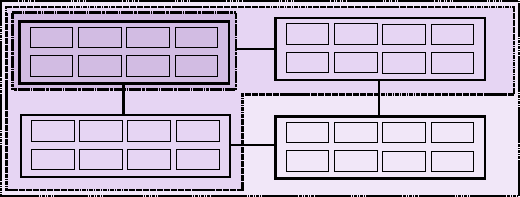
\psfig{file=NUMA.pdf,width =3in}
\caption{32-core machine with four NUMA nodes. It only takes two hops to get from any core to another node. The shades represent scheduling domains relative to the first core. From Lozi et al.~\cite{Lozi:2016}}
\label{fig:domains}
\end{figure}

For load balancing, cores exist in a hierarchy where each level is called a \emph{scheduling domain}. The groups within each level are based on how cores share resources within the machine. The lowest level of scheduling domain is a single core. In the machine described in Section~\ref{sec:cache} there were 32 cores. These cores represented the first level of scheduling domains. The second domains were determined by groups of eight adjacent processors which made four NUMA nodes. The third level was formed by groupings of nodes that are within one hop of each other. The final level was all of the nodes as one unit. See Figure~\ref{fig:domains}.~\cite{Lozi:2016}

\begin{figure}
\centering
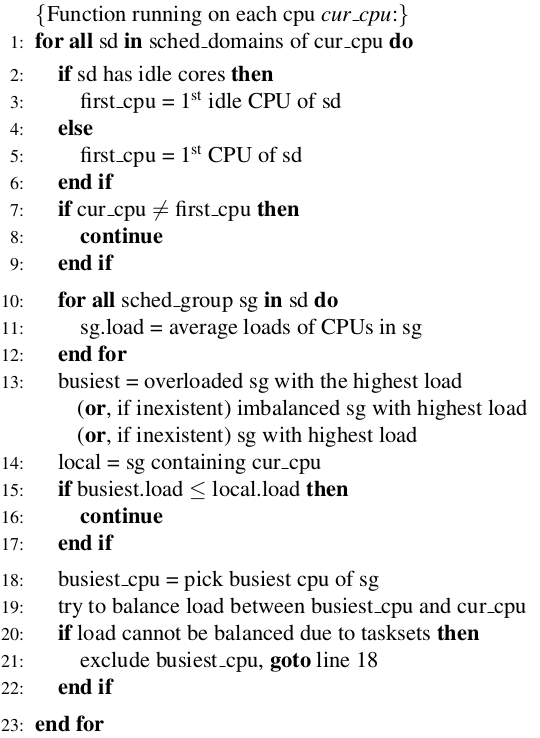
\psfig{file=CFS_Loadbalancer.png,width =3in}
\caption{Simplified CFS Load Balance algorithm from Lozi et al. CPUs are cores.~\cite{Lozi:2016}}
\label{fig:cfsloadbalancer}
\todo[inline]{Should make into an algorithm rather than figure.}
\end{figure}

A naiive approach to load balancing would be to compare load on each core and transfer tasks from cores with the highest load to cores with the lowest load. This approach would not put into consideration improving thread locality or NUMA. Instead, the CFS load-balancing algorithm is executed on each CPU for each scheduling domain that the CPU is a part of starting from the first level to last levels of scheduling domain. A simplification of the CFS load balancing algorithm can be found in Figure \ref{fig:cfsloadbalancer}.

In the CFS load balancer, one core per scheduling domain is responsible for performing the load-balancing for that domain. That core is either the first core that is idle or the first core of the scheduling domain (Lines 2-9). Then for each scheduling group within the scheduling domain, the average load is computed (Lines 10-12) and the group with the highest load is determined to be the busiest group (Line 13). If the busiest group is less busy than the group containing this CPU (local), then the load is considered balanced for this level and continues on to consider the next scheduling domain (Lines 14-17). At lines 18 to 23 the current core balances load between the bustiest core and itself.~\cite{Lozi:2016}

Several optmizations made the scheduler such that it runs the load balancing operation less often. Lines 2-8 is an example of this where if any of the cores are idle, the first idle core in the scheduling domain is chosen to consider load balancing. If all cores are busy, the first core of the scheduling domain is chosen. There is also a power optimization where idle cores don't run the load balancing algorithm until awoken by an overloaded core. To improve cache locality, when an idle thread is awoken by an active thread, the scheduler prefers to assign the awoken thread to the same core so that they share a last-level cache.~\cite{Lozi:2016}

\subsection{Bugs and Fixes for the CFS}
\label{sec:cfsbugs}

Now that we know how the load balancer functions, we will now dive into the bugs that occur as a result of the complex, strict requirements that have built up over time on the CFS.

\subsubsection{The Group Imbalance bug}
\label{sec:cfsfault_grpimbalance}

Lozi et al. found that the scheduler was periodically not balancing load due to two reasons. The hierarchical design and complexity of the load metric. The researchers were running a 64 threaded \emph{make} process simultaneously with a single threaded \emph{R} process. Because of group schedule features, the amount of load for each of the make threads are 1/64 of the one thread of the R process. On their system they observed that Two nodes were underloaded and should have been stealing work from more loaded cores on other nodes, but this did not happen. This is due to the hierarchical design of the load balancer. When the load balancer considers stealing threads, it does not consider the load of a single thread but rather the load of the whole group. In this case, the node with the R program had the same load as the node with the make process, so its node did not try to steal work from the node running make even though there were cores available.~\cite{Lozi:2016}

They fixed this problem by instead of defining load of a scheduling group as the average load of cores in the group, it is defined by the load of the core with the minimum load in the scheduling group. By fixing this issue, the efficiency of the R program remained the same, however the completion time of make decreased by 13 percent. On a certain parallel program within the NAS benchmark called lu, this bug fix improved performance by 13 times because the bug compounded lock contention by colocated threads.~\cite{Lozi:2016}

\subsubsection{The Scheduling Group Construction bug}
\label{sec:cfsfault_grpconstruct}

There is a function in Linux called taskset which allows an application to pin its threads to certain available cores. On certain machines, sequential NUMA nodes may be located more than one hop from each other. When Linux spawns new thread, they are created on the same node as the parent thread. The parent thread only exists on one core, so all spawned threads are made on the same node. The first scheduling group is constructed by all adjacent nodes to one node (say, Node 0), and following scheduling groups are constructed by adjacent nodes to nodes that were not in any of the previous groups. On a system it is possible for two nodes to be within one hop of the starting nodes of each group, but be two hops from each other. See Figure \ref{fig:cfs_schedgroups}.~\cite{Lozi:2016}

Within that system, the two scheduling groups constructed are {0,1,2,4,6} and {1,2,3,4,5,7}. Nodes 1 and 2 are two hops from each other but occur in both scheduling groups. When load balancing runs on Node 2 and it should steal work from an overloaded Node 1, it will look between the scheduling groups to compare which is lower. But both scheduling groups contain Node 1 and 2, so both scheduling groups' average load will be the same! Node 2 will never steal work.~\cite{Lozi:2016}

They fixed this bug by constructing scheduling groups relative to each core's own perspective. This allows nodes that are two hops away that should otherwise be able to share work to be a part of different scheduling groups and successfully contend for load balancing. Fixing this bug improved efficiency of 9 parallel programs in the NAS benchmark problems mostly by around 2 times, but for one problem, lu, up to 27 times. lu is an extreme example where all threads were being allocated only on one core.~\cite{Lozi:2016}

\begin{figure}
\centering
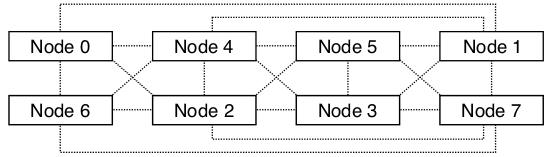
\psfig{file=CFS_AdjacentNodes.png,width =3in}
\caption{8-node AMD Bulldozed machine from Lozi et al.~\cite{Lozi:2016}}
\label{fig:cfs_schedgroups}
\end{figure}

\subsubsection{The Overload-on-Wakeup bug}
\label{sec:cfsfault_overload}


The optimization where threads that are awakened by other threads are placed on the same core for improved cache locality, this becomes a problem when the core with the requesting thread is already overloaded. The thread will join the runqueue on this busy core rather than consider being migrated to an idle core elsewhere. For some workloads this is acceptable, but simply making the most of cache isn't always the best decision. This bug occurs primarily on database systems. The following sequence of events will illustrate how the Overload-on-Wakeup bug occurs.~\cite{Lozi:2016}

	Consider two nodes running on a database system. Node A and Node B both have a database thread. A transient thread is created by the kernel on Node A for some background function such as system logging. During this time, the load balancer detects that the node is overloaded, and decides to migrate a thread to Node B. If it decides to move the transient thread, that will pose no issue for performance. If it migrates the database thread, two database threads, which sleep and awaken frequently, will be running on the same node. The scheduler does not differentiate between cores that are idle for a short time versus a long time, so when the scheduler considers thread migration destinations, it might see a Node, which happens to have a database thread that is currently idle, and decide that the node needs more work.~\cite{Lozi:2016}

Lozi et al. fixed this bug by modifying the thread wake up code. The scheduler first checks to see if the core that the thread was already assigned to is idle. If it is, then wake up the thread on that core. If the power manager policy of the system is set up so that cores never enter low-power mode and there are idle cores, the scheduler chooses the core that has been idle for the most time and assigns the thread to that core. This fix is only relevant to workloads where threads frequently sleep. The scheduler already provides a list of cores that are idle, so choosing the core that has been idle the longest takes constant time. Their fix improves performance by 13.2\% on a full TPC-H database workload but up to 22.2\% for certain queries.~\cite{Lozi:2016}

\subsubsection{The Missing Scheduling Domains bug}
\label{sec:cfsfault_missingsched}

This bug is actually something that was already fixed but regressed on Linux kernel version 3.19 (and later) when an important line of code was removed in a refactor that causes the system to misrepresent the amount of scheduling domains that are available for assigning threads to. This ended up causing load-balancing to never happen, meaning processes, subprocesses and their threads to stop looking for other NUMA nodes to assign themselves to. Nodes that do not have any threads will never receive threads and nodes that do have threads will accumulate all of the spawned threads.

This bug required that one of the cores become disabled and re-enabled. So while rare, reintroducing the removed line of code increased efficiency in a certain tested program by a maximum of 138 times.~\cite{Lozi:2016}

\subsection{Shuffler}
\label{sec:shuffler}

Research by Kumar, Rajiv, Laxmi and Bhuyan studied 20 certain parallel algorithms and found that with many of them, adding more threads began to degrade program performance rather than improve. The researchers monitored time spent acquiring locks and number of LLC misses experienced while running these programs. They identified the source of this problem to be \emph{lock contention}.

Lock contention can be found in multithreaded programs where many threads compete for access to the same lock. Lock contention between threads in a program that reside on different processors leads to a higher than average LLC miss rate. This occurs because the thread requesting the lock also tends to be working on the same data, and the data would need to be refreshed on the requesting processor's cache if another processor had changed the data. If the threads of that multithreaded program were prioritized to be placed on one processor, then the program would experience a lower LLC miss rate. Neither the CFS nor the Solaris scheduler differentiate between threads of a single-threaded program versus the threads of a multithreaded program. This prevents the scheduler from using that metadata in its thread distribution mechanism. The following thread scheduler named \emph{Shuffler} by Kumar et al. takes this into account. The Shuffling framework was designed for multiprocessor multicore NUMA systems, and implemented on a 64-core 4-processor machine running Oracle Solaris 11.~\cite{KumarEtal:2014}

The Shuffling approach is for the scheduling algorithm to take into account what threads are contending for locks on what processors and migrate \textbf{whole threads} (rather than lock and cache) such that they share processors. The Shuffling Framework operates as seen in Algorithm \ref{alg:shuffler}. Threads that are reported to have higher lock acquisition times are threads that are requesting locks from outside of their processor. These are the threads that should be migrated to share processors. Details on the shuffling framework are as follows.~\cite{KumarEtal:2014}

\begin{algorithm}
	\SetKwInOut{Input}{input}\SetKwInOut{Output}{output}
	\Input{N: Number of threads;\\
	C: Number of Processors.}

	\Repeat{application terminates}{
		$\textbf{i. Monitor Threads}$ -- sample lock times of N threads.\\
		\If{lock times exceed threshold}{
			$\textbf{ii. Form Thread Groups}$ -- sort threads according to lock times and divide them into C groups. \\
			$\textbf{iii. Perform Shuffling}$ -- shuffle threads to establish newly computed thread groups.
		}
	}			

	\caption{The Shuffling Framework
	as presented in Kumar et al.~\cite{KumarEtal:2014}}\label{alg:shuffler}
\end{algorithm}

\begin{description}
\item [Monitor Threads] \ \\
First, we monitor the amount of time user threads spend acquiring locks and store it in a data structure. 

\item [Form Thread Groups] \ \\
If sampled lock times exceed a certain threshold, threads are sorted by their lock acquisition times and grouped by their order in the sorted data structure. There are as many groups as processors that will be used to run the program. This procedure is run every 200 ms to continue to form groups of threads that should share processors.

\item [Perform Shuffling] \ \\
On an iteration of the shuffling procedure (every 500 ms), shuffling checks to make sure that if any threads aren't on processors that they were grouped to, they are migrated. Threads that are already on the processor that they were assigned to do not migrate. If the way that threads interacted with eachother doesn't change, the shuffling step is effectively skipped.~\cite{KumarEtal:2014}
\end{description}

Now that we know how the Shuffling Framework works, let's review the results that implementing it gives us.

\subsubsection{Shuffler Performance}
\label{sec:shuf_performance}

Figure \ref{fig:shuf_performance} details the improvements that Shuffling made relative to the default Solaris scheduler and three other schedulers. A positive number denotes that that scheduler was that more efficient than the default Solaris scheduler for that program. Each of the programs are multithreaded. The one they highlight the most was the Body Tracking (BT) algorithm of whose performance improved by 54 percent.~\cite{KumarEtal:2014} Figure \ref{fig:shuf_vs_solaris} compares the efficiency of Shuffler versus Solaris for the 20 same multithreaded programs.
\begin{figure}
\centering
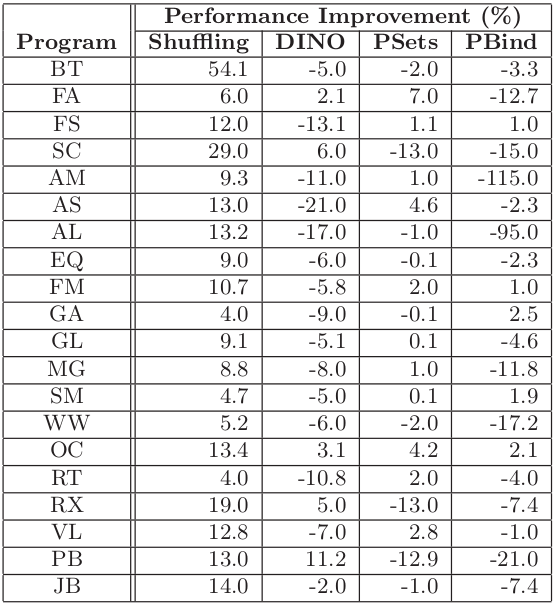
\psfig{file=Performance_Shuffler.png,width =3in}
\caption{Performance Improvements relative to Solaris across 20 multithreaded programs. From Kumar et al.~\cite{KumarEtal:2014}}
\label{fig:shuf_performance}
\todo[inline]{Should be a "table" not a figure}
\end{figure}

\begin{figure}
\centering
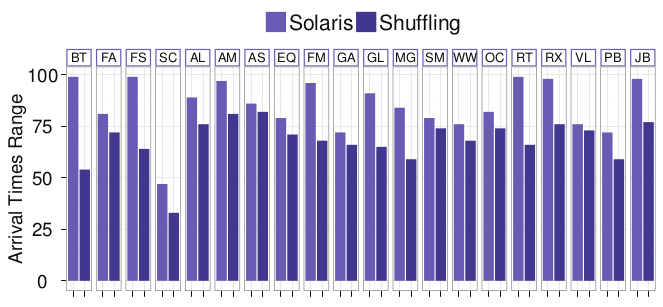
\psfig{file=SolarisVsShuffling.png,width =3in}
\caption{Lock arrival times ranges with Solaris vs. Shuffling. From Kumar et al.~\cite{KumarEtal:2014}}
\label{fig:shuf_vs_solaris}
\end{figure}

We just saw that lock contention is a problem for multithreaded parallel programs. Next we will cover a scheduler that takes a different approach to alleviating the lock contention problem. The designers of FLSCHED claim it is lockless, reduces context switches, and makes more efficient scheduling decisions than CFS.~\cite{JoEtal:2017}

\subsection{FLSCHED for Xeon Phi Manycore Processor}
\label{sec:flsched}

Manycore processors continue become more powerful and as such, more popular. The latest manycore processor as of September 2 2017, the latest version of Xeon Phi, has up to 76 physical cores where each core has small cache. The amount of cores a processor has is expected to increase given the popularity and importance of highly-parallel algorithms such as machine learning. The CFS was not built for this degree of parallelism. As the number of cores increase the negative impact of lock contention on the scheduler performance increases exponentially. As well, the cost of context switching continues to increase as hardware becomes capable of solving larger problems.

The context switch overhead for the Xeon Phi is larger than usual processors because it contains additional vector-processing register sets. \cite{JoEtal:2017} A machine that supports vector processing allows one to perform instructions on vectors of data rather than scalars~\cite{Mellon}. The Xeon Phi comes in many sizes. The Xeon Phi processor used by FLSCHED researchers Jo, Kang, Min, and Kim had 57 cores. ~\cite{JoEtal:2017}

\subsubsection{``Lockless'' Thread Scheduler}
\label{sec:flsched_about}

The design goals for the CFS differ from the FLSCHED. The CFS was designed with different requirements in mind than FLSCHED. The CFS was designed with responsiveness, fairness and load-balancing in mind because it was intended for Desktop and Server use. The FLSCHED was designed strictly with efficiency in mind so responsiveness and fairness are not important. A great deal of state information is considered in the choice of what threads run and when. Since FLSCHED was intended for manycore parallel machines, it is more impactful to simply make descisions faster rather than more purposefully.~\cite{JoEtal:2017}

The CFS implementation has 11 locks which are used for load balancing mechanisms, runqueue management, runtime statistics updates, and addition scheduler features. FLSCHED removes runtime statistics entirely from the scheduler because it does not depend on them to make decisions. FLSCHED does not use periodic load balancing, does not provide the feature to limit maximum CPU bandwidth, nor any of the CFS group features. While the FLSCHED substitutes for the CFS, it does still run on top of the scheduler core which has locks. Context switches on FLSCHED must be requested by setting a bit in the scheduler. Responses to context switch requests are delayed on purpose to minimize the number of context switches.~\cite{JoEtal:2017}

Timeslices in FLSCHED are assigned Round-Robin. The only managed scheduling information is the timeslices that threads receive. Thread preemption in FLSCHED mostly occurs because there is another thread with a higher priority. Rather than immediately preempting the running thread to replace with the new thread, FLSCHED reorders runqueues such that the important thread will come next after a normal task switch.~\cite{JoEtal:2017}

\todo[inline]{define Round-Robin scheduling, which might enlighten us what is done to execute the runqueues.}

\subsubsection{FLSCHED Perfomance}
\label{sec:flsched_performance}

To evaluate FLSCHED performance, researchers used the NAS Parallel Benchmark (NPB), a set of programs that are used to evaluate the efficiency of parallel computing systems. NPB version 3.3.1 consists of 10 problems, but two of which can not run on the Xeon Phi due to memory constraints. The tests were ran on FLSCHED, the CFS, and two other schedulers by the names FIFO and RR in order to compare. From the results of these tests (Figure \ref{fig:flsched_npb}), you can see that the FLSCHED scales better as the number of threads increases for six out of eight problems. Efficiency of the ep and is programs did not improve under FLSCHED. \cite{JoEtal:2017}

\begin{figure*}
\centering
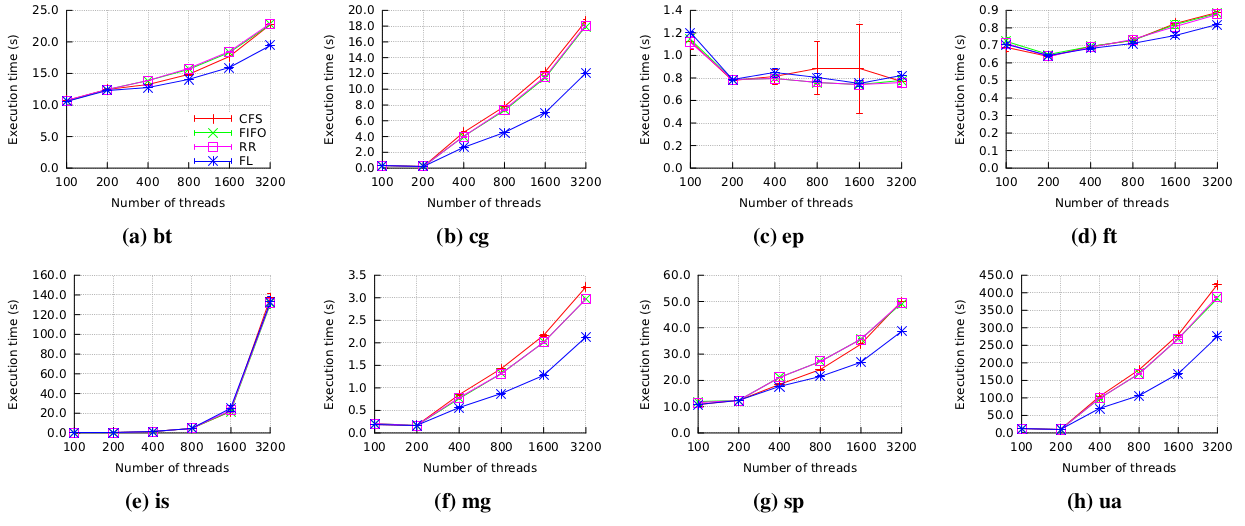
\psfig{file=FLSCHED_NPBCMP.png,width =5.1in}
\caption{FLSCHED performance comparison of various schedulers on programs in the NAS Parallel Benchmark. From Jo et al.~\cite{JoEtal:2017}}
\label{fig:flsched_npb}
\end{figure*}


The researchers traced the cause of the efficiency improvements to minimizing a certain kind of lock called a spin lock from their scheduler. Figure \ref{fig:flsched_spinlock} shows the percent of time that each of these schedulers spend processing spin locks. Time spent on spin locks was more than halved for programs cg, mg, sp and ua. \cite{JoEtal:2017}

\begin{figure}
\centering
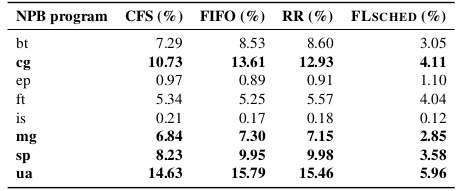
\psfig{file=FLSCHED_SpinLock.png,width =3in}
\caption{ Percent of time that various schedulers spend executing a certain type of lock called a spin lock. Lock times were measured throughout the runtime of the NAS Parallel Benchmark at 1,600 threads. From Jo et al.~\cite{JoEtal:2017}}
\label{fig:flsched_spinlock}
\todo[inline]{Should be a "table" not a figure}
\end{figure}

Finally, Jo et al. also measured per-function diagnostics of both the CFS and FLSCHED using ftrace. The functions measured were crucial scheduler tasks. The CFS was compared to FLSCHED by running hackbench, a well known scheduler stress test, and measuring number of function calls and time spent executing them. See Figure \ref{fig:flsched_func}.\cite{JoEtal:2017}

\begin{figure*}
\centering
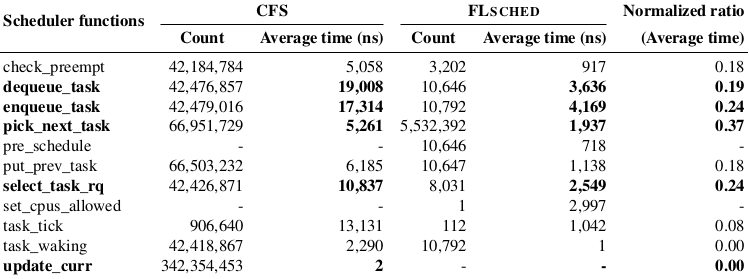
\psfig{file=FLSCHED_SchedulerCMP.png,width =5.3in}
\caption{Average time and function call counts for critical scheduler tasks. The numbers were gathered using ftrace while running the hackbench stress test for thread schedulers. From Jo et al.~\cite{JoEtal:2017}}
\label{fig:flsched_func}
\todo[inline]{Should be a "table" not a figure}
\end{figure*}

\todo[inline]{FLSched source does not specify what kind of memory constraints disable those two parallel problems from being run on the Xeon Phi. What's stopping you from just attaching more RAM..? Is there some restriction on memory emplaced by using the Xeon Phi? The Xeon Phi is not a normal processor, the researchers appear to be interfacing with this processor through a primary system, so maybe it doesn't use ram and only has built-in memory or something..?}

\section{Conclusions}
\label{sec:conclusions}

Most of the improvements to the CFS in Section 3.2 improves user experience and system efficiency for Linux systems that use the CFS. The Shuffler makes multicore multiprocessor systems function more efficienct than under the CFS. The FLSCHED makes manycore parallel machines intended for problem-solving more efficient by removing extraneous features.

\todo[inline]{I'm not sure yet how to properly approach pulling these three different technologies together to a good conclusion.}

\section*{Acknowledgments}
\label{sec:acknowledgments}


% The following two commands are all you need in the
% initial runs of your .tex file to
% produce the bibliography for the citations in your paper.
\bibliographystyle{abbrv}
\bibliography{scheduling}  
% Remember to run:
% latex bibtex latex latex
% to resolve all references

\end{document}
